\documentclass[10pt,a4paper]{article}
\usepackage[margin=2.1cm]{geometry}
\usepackage{amsmath,amssymb,booktabs,graphicx,tikz,xcolor,enumitem,microtype,url,float}
\usepackage[section]{placeins}
\urlstyle{tt}
\usepackage[colorlinks=true,linkcolor=blue!50!black,urlcolor=blue!50!black,citecolor=blue!50!black]{hyperref}
\usetikzlibrary{positioning,arrows.meta}
\setlength{\parskip}{3pt plus 1pt}
\setlength{\parindent}{0pt}
\newcommand{\relu}{\operatorname{ReLU}}
\newcommand{\sgn}{\operatorname{sign}}
\newcommand{\E}{\mathbb{E}}
\newcommand{\R}{\mathbb{R}}
\definecolor{L0}{HTML}{2a78d6}\definecolor{L1}{HTML}{eb6834}\definecolor{L2}{HTML}{1baf7a}\definecolor{L3}{HTML}{eda100}\definecolor{CUE}{HTML}{6250d6}
\title{\vspace{-1.2cm}Layers as lenses: how a two-hidden-layer ReLU network\\ learns an oblique decision tree, step by step\\[2pt] {\large A handout for new collaborators}}
\author{Harish G.\ and collaborators \quad (\texttt{layer-lenses} repository, October 2026)}
\date{}
\begin{document}
\maketitle
\vspace{-0.9cm}
\begin{abstract}\noindent
We study how gradient descent builds a hierarchy of features. The task is a depth-5 oblique decision tree (ODT) on the unit sphere in $\R^{100}$: 15 internal nodes with orthonormal normals route each input to one of 16 label nodes, where the label is the sign of a sixteenth normal. The network is a 62--60--1 ReLU network without biases. The central idea is that every first-layer row sees the data \emph{through a lens}: the active region of the units that read it. Its gradient is the gradient of a linear classifier on data reweighted by that lens, so a row learns whatever direction the lens makes informative. We design an initialisation in which no row contains any internal normal and all the information about the tree sits in the wiring of the second layer, and we show that plain SGD then discovers the 15 internal normals level by level, builds 32 leaf detectors, and reaches 0.4\,\% test error. A symmetrised gradient turns the same runs into a simulation of population gradient flow, which separates the deterministic mechanism from symmetry breaking by sampling noise. This handout gives the definitions, the design, the learned representation, and the main trajectories, all from saved runs in the repository.
\end{abstract}

\section{The output of a ReLU network as a sum over paths}
Consider a network with two hidden layers and no biases, $f(x) = W_{\mathrm{out}}\,\relu\!\big(W_2\,\relu(W_1 x)\big)$, with $W_1\in\R^{62\times 100}$, $W_2\in\R^{60\times 62}$, $W_{\mathrm{out}}\in\R^{1\times 60}$. Write $w_r$ for row $r$ of $W_1$ and let $g_r(x)=\mathbf 1[w_r\cdot x>0]$ and $g_u(x)=\mathbf 1[(W_2\relu(W_1x))_u>0]$ be the gates. Because $\relu(z)=g(z)\,z$,
\begin{equation}
f(x)\;=\;\sum_{u=1}^{60}\sum_{r=1}^{62} W_{\mathrm{out},u}\, g_u(x)\, W_{2,ur}\, g_r(x)\, (w_r\cdot x)
\;=\;\sum_{(u,r)} \underbrace{W_{\mathrm{out},u} W_{2,ur}}_{\text{path weight}}\;\underbrace{g_u(x)g_r(x)}_{\text{path gate}}\;(w_r\cdot x).
\label{eq:paths}
\end{equation}
The output is a sum over \emph{paths} $(u,r)$; each path is a linear function of $x$ switched on inside a region of input space, the intersection of the active regions of its two units. The function is piecewise linear and positively homogeneous of degree 3 in the parameters.

\begin{figure}[!htbp]\centering
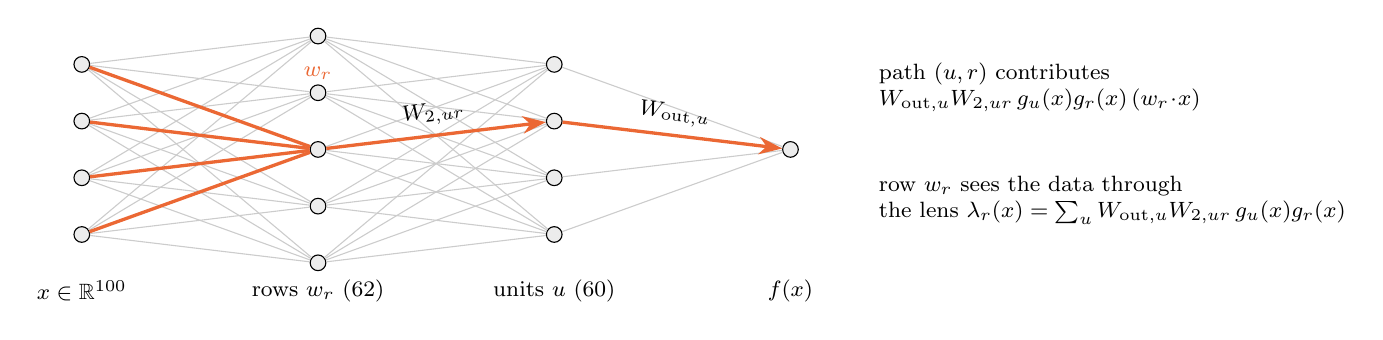
\begin{tikzpicture}[x=1cm,y=0.72cm,>=Stealth,font=\footnotesize]
\foreach \i in {1,...,4}{\node[circle,draw,inner sep=2pt,fill=gray!15] (x\i) at (0,-\i) {};}
\node at (0,-5) {$x\in\R^{100}$};
\foreach \i in {1,...,5}{\node[circle,draw,inner sep=2pt,fill=gray!15] (r\i) at (3,-\i+0.5) {};}
\node at (3,-5) {rows $w_r$ (62)};
\foreach \i in {1,...,4}{\node[circle,draw,inner sep=2pt,fill=gray!15] (u\i) at (6,-\i) {};}
\node at (6,-5) {units $u$ (60)};
\node[circle,draw,inner sep=2pt,fill=gray!15] (o) at (9,-2.5) {};
\node at (9,-5) {$f(x)$};
\foreach \i in {1,...,4}{\foreach \j in {1,...,5}{\draw[gray!40] (x\i)--(r\j);}}
\foreach \i in {1,...,5}{\foreach \j in {1,...,4}{\draw[gray!40] (r\i)--(u\j);}}
\foreach \i in {1,...,4}{\draw[gray!40] (u\i)--(o);}
\draw[very thick,L1,->] (r3)--(u2) node[midway,above,sloped,black] {$W_{2,ur}$};
\draw[very thick,L1,->] (u2)--(o) node[midway,above,sloped,black] {$W_{\mathrm{out},u}$};
\foreach \i in {1,...,4}{\draw[very thick,L1] (x\i)--(r3);}
\node[L1,fill=white,inner sep=1pt] at (3.0,-1.15) {$w_r$};
\node[align=left,anchor=west] at (10,-1.4) {path $(u,r)$ contributes\\ $W_{\mathrm{out},u}W_{2,ur}\,g_u(x)g_r(x)\,(w_r\!\cdot\! x)$};
\node[align=left,anchor=west] at (10,-3.4) {row $w_r$ sees the data through\\ the lens $\lambda_r(x)=\sum_u W_{\mathrm{out},u}W_{2,ur}\,g_u(x)g_r(x)$};
\end{tikzpicture}
\caption{The path decomposition \eqref{eq:paths}. A row's gradient is a linear-classifier gradient on data reweighted by the lens $\lambda_r$.}
\label{fig:paths}
\end{figure}

\paragraph{Gradient of a row.} For the logistic loss $\ell(y,f)=\log(1+e^{-yf})$ the population gradient with respect to $w_r$ is
\begin{equation}
-\nabla_{w_r}\,\E\,\ell\;=\;\E\big[\sigma(-yf(x))\,y\,\lambda_r(x)\,x\big],\qquad
\lambda_r(x)=\sum_u W_{\mathrm{out},u} W_{2,ur}\, g_u(x)\, g_r(x).
\label{eq:lens}
\end{equation}
This is the gradient of a \emph{linear} classifier $w_r\cdot x$ on the data reweighted by $\sigma(-yf)\lambda_r(x)$. The weight $\lambda_r$ is what we call the row's lens: it is set by the units that read the row (their readout, their weight on the row, and their active region) and by the row's own gate. At initialisation $f\approx 0$ and $\sigma(-yf)\approx\tfrac12$, so a row moves along $\sum_u W_{\mathrm{out},u}W_{2,ur}\,\E[g_u g_r\, y\, x]$. Everything in this handout follows from asking what $\E[g_u g_r\,y\,x]$ is for the ODT data and for the units we build.

\section{The data: a depth-5 oblique decision tree}
Inputs are uniform on the unit sphere in $\R^{100}$. A fixed set of 31 orthonormal vectors $u_0,\dots,u_{30}$ (drawn once, tree seed 5178) is arranged as a complete binary tree in heap order (Figure~\ref{fig:tree}): node $j$ has children $2j+1$ and $2j+2$. An input descends from the root: at internal node $j$ it goes to $2j+1$ if $u_j\cdot x<0$ and to $2j+2$ otherwise. After four decisions it reaches a label node $m\in\{15,\dots,30\}$ and the label is $y=\sgn(u_m\cdot x)$. We call the 15 internal normals \emph{routing normals} and the 16 others \emph{leaf normals}; the region of inputs that reaches label node $m$ is the \emph{leaf cell} of $m$, each of probability $1/16$. The label is noiseless, so the Bayes error is 0, and the task is invariant under every tree flip (negate $u_j$ and exchange the two subtrees below $j$), under rotations of the 69-dimensional orthogonal complement of the normals, and anti-invariant under negating all 16 leaf normals (which negates $y$). All runs use $10^7$ training points per epoch in minibatches of $10^4$ (1000 steps per epoch) and a fixed test set of $2\times10^5$ points.

\begin{figure}[!htbp]\centering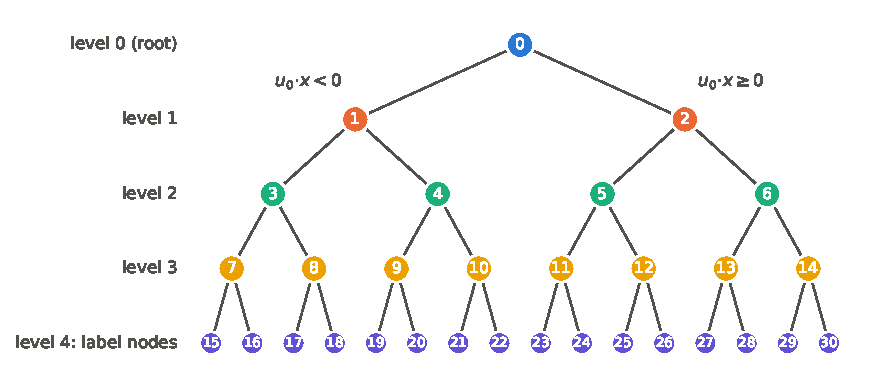
\includegraphics[width=0.9\textwidth]{figs/tree.pdf}
\caption{The tree. Internal nodes $0$--$14$ route with the routing normals (colours mark the levels used throughout: \textcolor{L0}{level 0}, \textcolor{L1}{level 1}, \textcolor{L2}{level 2}, \textcolor{L3}{level 3}); label nodes $15$--$30$ (\textcolor{CUE}{violet}) carry the leaf normals that set the label.}
\label{fig:tree}
\end{figure}

\paragraph{What a linear model sees.} The best linear classifier is a useful reference. By strict convexity and the symmetries above, its population optimum is exactly $c\,v$ with $v=\sum_{m=15}^{30}u_m$, the sum of the leaf normals: every routing component and every off-span component is forced to zero. Numerically $c\approx1.05$, the loss is $0.672$ (against $\log 2=0.693$) and the error is $41.9\,\%$. The direction $v$ matters below: it is the direction a row converges to when its lens is uninformative, and the designed cues are built around it.

\section{The network and the designed initialisation}
\paragraph{Architecture.} 62 first-layer rows, 60 second-layer units, one output, no biases, plain SGD on the logistic loss with learning rate $0.1$ and a cosine schedule to $0.005$ over the run. The rows have two roles fixed at initialisation:
\begin{itemize}[leftmargin=1.4em,itemsep=1pt]
\item \textbf{30 probes}, one per (internal node $j$, pole $\pm$). Each probe is $\sqrt2$ times a unit vector in the orthogonal complement of all 31 normals, the 30 directions being mutually orthogonal. A probe therefore starts with \emph{no component on any tree normal}: it is pure noise with respect to the task.
\item \textbf{32 cues}, one per (label node $m$, pole $\pm$): $\pm\sqrt2\,(v+\beta u_m)/\|v+\beta u_m\|$ with $\beta=1$. A cue is the linear-model direction $v$ with a bias towards its own leaf normal; its cosine with $u_m$ is $0.46$ and with every other leaf normal $0.23$.
\end{itemize}
The second layer has four units per internal node $j$ (60 units for 15 nodes), with a block sign $b$ and a path sign $s\in\{\pm1\}$, the four types $(b,s)\in\{(+,+),(+,-),(-,-),(-,+)\}$. Each unit:
\begin{itemize}[leftmargin=1.4em,itemsep=1pt]
\item \textbf{vetoes one probe of its node}: weight $-1$ on the probe of pole $\sgn(bs)$. With $\relu$ this cannot do anything until the probe carries a direction; it is where the probe's gradient enters.
\item \textbf{reads the cues with a side contrast} (run 60's design, Figure~\ref{fig:init}): weight $s\cdot\mathrm{pole}\cdot c_l$ on the cues of the leaves under $j$ on one side (the ``open'' side) and $-s\cdot\mathrm{pole}\cdot c_l$ on the other side, nothing outside the subtree, with $c_l=2^{-(5-l)/2}$ for a node of level $l$ ($0.18, 0.25, 0.35, 0.5$).
\item has readout $s\times0.8165$. The readout's learning rate is multiplied by 80 (this replaces a third layer used in earlier runs).
\end{itemize}
Run 70 uses the same rows but ``majority'' cue weights ($0.2$ on the open side, $0.1$ on the vetoed side, $0.1$ outside, all times $s\cdot\mathrm{pole}$), an extra $+1$ link to the partner probe of the vetoed one, and no readout speed-up. The whole family is parametrised by thirteen scalars $\alpha_1,\dots,\alpha_{13}$ (row norms, cue bias, the three cue weights, the two probe links, the two readout sizes, two learning-rate scales, and the cues' in-span fraction) in \texttt{layer\_lenses.alpha\_init}.

\begin{figure}[!htbp]\centering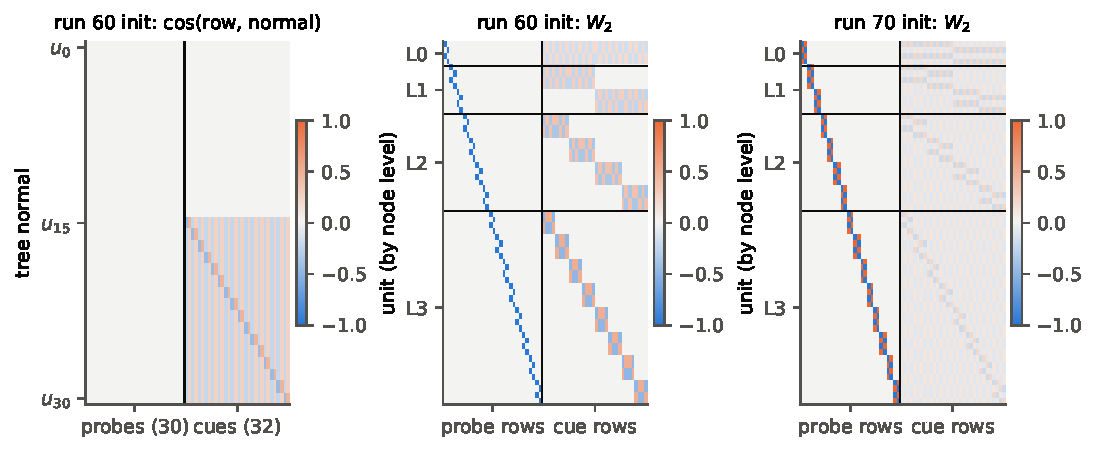
\includegraphics[width=\textwidth]{figs/init_run60_70.pdf}
\caption{The initialisation. Left: cosines of the 62 rows of $W_1$ with the 31 normals in run 60. The probes have none; each cue has $0.46$ on its own leaf normal and $\pm0.23$ on the other fifteen (the sign is the cue's pole). Middle: $W_2$ of run 60, units grouped by the level of their node. The diagonal of $-1$ entries on the probe rows is the vetoes; the block pattern on the cue rows is the side contrast, with magnitude growing with the level. Right: $W_2$ of run 70 (majority weights, partner links).}
\label{fig:init}
\end{figure}

\paragraph{Why these initialisations are interesting.} Nothing in the first layer knows the 15 routing normals: the probes are random off-span directions, and the cues only know their own leaf. The tree is encoded in \emph{which cues each unit reads and with which sign}. By \eqref{eq:lens}, the probe vetoed by unit $u$ receives the push $W_{\mathrm{out},u}W_{2,u p}\,\E[g_u\, y\, x]$ once it has any direction at all, and $\E[g_u\,y\,x]$ restricted to a leaf cell $m$ has a component along every routing normal $a$ above $m$, with the sign of the side of $a$ on which $m$ lies. A unit whose cue weights favour the leaves on one side of node $j$ has an active region biased to that side, so the push on its probe along $u_j$ is $\propto\sum_{m\text{ under }j}\mathrm{side}_j(m)\,p_u(m)$, where $p_u(m)$ is the probability that the unit is active on cell $m$. The side contrast of the design makes this sum large; a unit that reads both sides equally pushes nothing along $u_j$ (this is the failure of run 68, not shown). The same formula gives a push along every ancestor of $j$, which is why the probes acquire a transient ancestor component (Figure~\ref{fig:traj60}, middle). The init is also an exact fixed point of the tree symmetries, which is what makes Section~\ref{sec:sym} possible, and it is small enough that every quantity in the trajectory can be read off.

\section{Results of runs 60 and 70}
Both runs train in two phases: the cue rows are frozen for the first 500 epochs (so the probes learn with a fixed lens), then everything is free for 500 more. Table~\ref{tab:results} and Figures~\ref{fig:traj60}--\ref{fig:traj70} summarise them.

\begin{table}[!htbp]\centering\footnotesize\setlength{\tabcolsep}{4pt}
\begin{tabular}{llcccccl}
\toprule
run & init, optimiser & \multicolumn{4}{c}{probe capture epoch, by level} & cues & loss / error / nodes\\
 & & L0 & L1 & L2 & L3 & rotated by & at the end\\
\midrule
60 & run 60 design, SGD & 10 & 40 & 22 & 31 & 653 & 0.019 / 0.40\,\% / 31 of 31\\
70 & run 70 design, SGD & 99 & -- & -- & -- & -- & 0.140 / 4.0\,\% / 19 of 31\\
\midrule
74 & run 60 design, symmetrised & 9 & 15 & 21 & 30 & 801 & 0.029 / 0.45\,\% / 31 of 31\\
114 & as 74, cosine restarted at epoch 500 & 10 & 39 & 22 & 30 & 598 & 0.006 / 0.05\,\% / 31 of 31\\
73 & run 70 design, symmetrised, 1000 frozen + 500 & 98 & 408 & 313 & 396 & -- & 0.111 / 2.3\,\% / 15 of 31\\
97 & run 73 continued 2000 epochs, fresh cosine & \multicolumn{4}{c}{(already captured)} & 1523 & 0.010 / 0.11\,\% / 31 of 31\\
\bottomrule
\end{tabular}
\caption{Capture = first epoch at which every probe of the level has $|\cos|>0.95$ with its own routing normal; ``nodes'' counts the normals covered by some row at the end. Run 97's epochs are counted from the start of run 73.}
\label{tab:results}
\end{table}

\begin{figure}[!htbp]\centering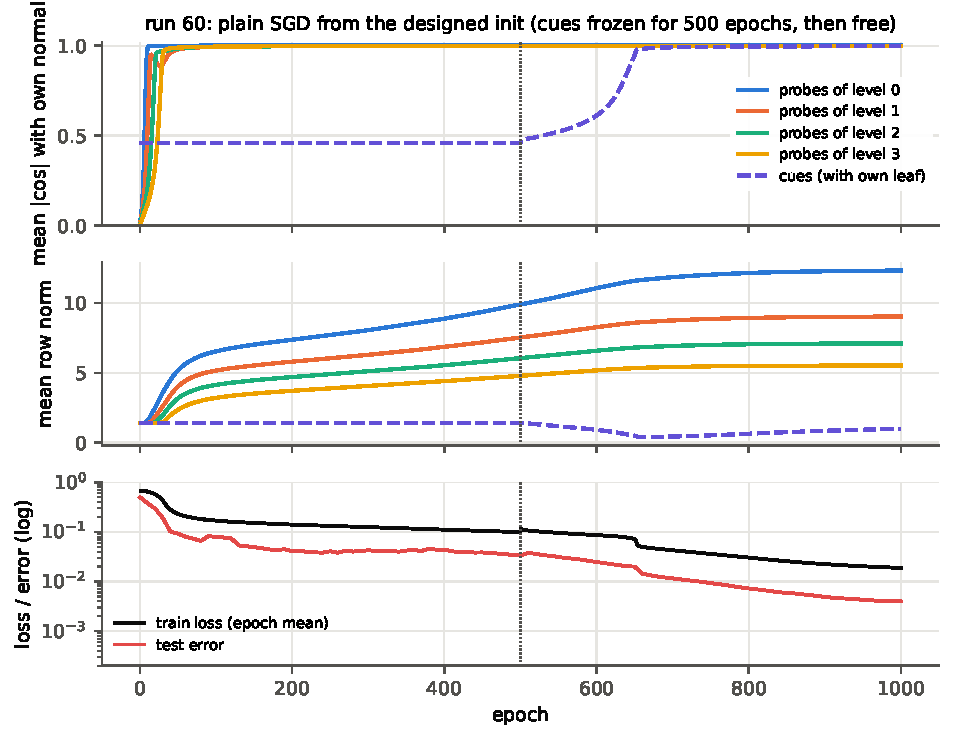
\includegraphics[width=0.9\textwidth]{figs/traj_run60.pdf}
\caption{Run 60. Top: mean $|\cos|$ of the probes with their own routing normal, by level, and of the cues with their own leaf normal. The probes are captured within 10--40 epochs, root first; the cues (frozen until epoch 500, dotted line) rotate from $0.46$ to $1$ during the free phase. Middle: row norms grow level by level (root largest). Bottom: training loss and test error; the drop at epoch 650 is the cue rotation.}
\label{fig:traj60}
\end{figure}

\begin{figure}[!htbp]\centering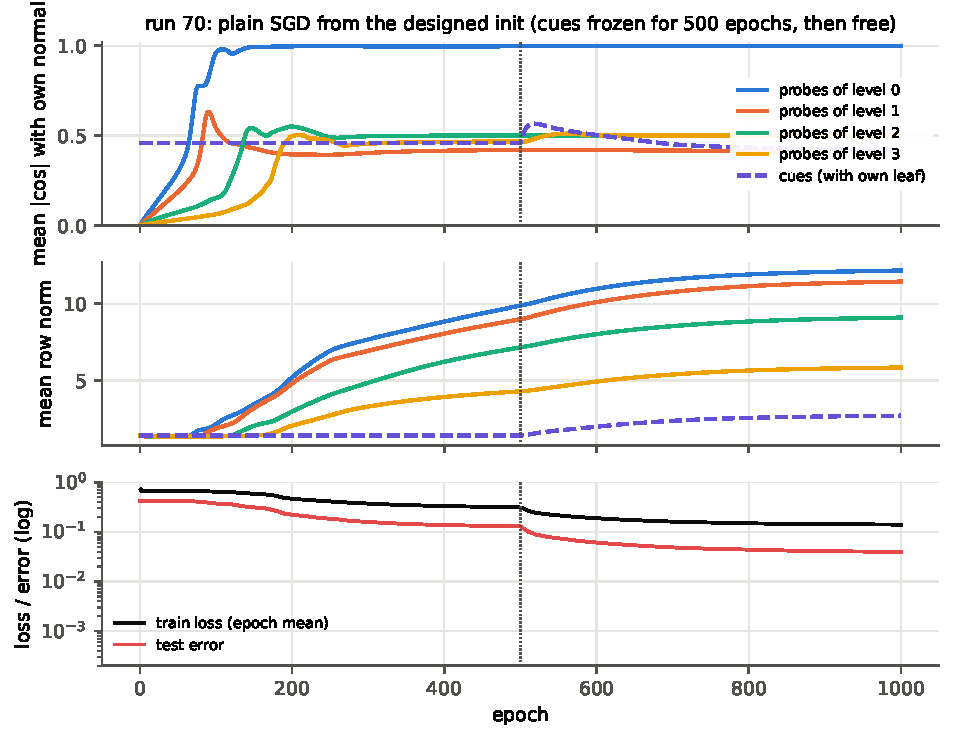
\includegraphics[width=0.9\textwidth]{figs/traj_run70.pdf}
\caption{Run 70 (majority cue weights, partner links, no readout speed-up). Only the root is captured cleanly; the probes of levels 1--3 end at $|\cos|\approx0.4$--$0.5$ with their own node because several of them go to the root or to an ancestor instead. The cues never rotate and the loss floors at $0.14$. Section~\ref{sec:sym} shows that this is sampling noise breaking the symmetry, not a defect of the design.}
\label{fig:traj70}
\end{figure}

\section{How the tree is represented in the trained network}
\label{sec:rep}
Figure~\ref{fig:learned} shows run 60 at epoch 1000, and Figure~\ref{fig:unit} one unit. The representation is explicit:
\begin{enumerate}[leftmargin=1.4em,itemsep=1pt]
\item \textbf{The first layer is a feature bank of the normals.} Each probe has become $\pm u_j$ for its node (the two probes of a node carry the two poles), with norms $12.3, 9.0, 7.1, 5.5$ by level; each cue has rotated to $\pm u_m$ with norm $\approx1$. The off-span part of every row has gone. A row of the form $\|w\|\,\relu(\pm u_j\cdot x)$ is a half-space detector for one side of one node.
\item \textbf{Units are $\relu(\text{background}-\text{vetoes})$.} A level-3 unit (node $j$ of level 3, leaf $m$ below it) has weight $\approx-6$ on its own probe and $\approx-5$ on one probe of each of its three ancestors (Figure~\ref{fig:unit}: unit 28 of node 7 vetoes $u_7$, $u_3$, $u_1$, $u_0$), a veto of $-4$ on the opposite-pole cue of its leaf, and small positive weights on the other cues. The vetoes switch the unit off whenever $x$ is on the wrong side of any ancestor, so the unit is active on 3.9\,\% of the inputs and 96\,\% of its active inputs lie in a single leaf cell: it is a \emph{leaf-cell detector}, and inside the cell its output follows $\sgn(u_m\cdot x)$ through the cues.
\item \textbf{The level-3 units carry the function.} Their readouts are $\pm62$ on average against $4.4$ at level 0; removing the 28 units of levels 0--2 raises the test error only from $0.40$ to $0.77\,\%$, while removing the 32 level-3 units raises it to $24.8\,\%$. On each leaf cell the logit is a sum of $\relu(\pm u_m\cdot x)$ terms with the right signs, which is the ODT itself. The units of levels 0--2 are the \emph{scaffold}: they are the units that pushed the probes of their own node (a level-3 unit has no weight on an ancestor's probe at init, so it cannot create the ancestor's feature, only use it), and they become dispensable once the features exist.
\end{enumerate}

\begin{figure}[!htbp]\centering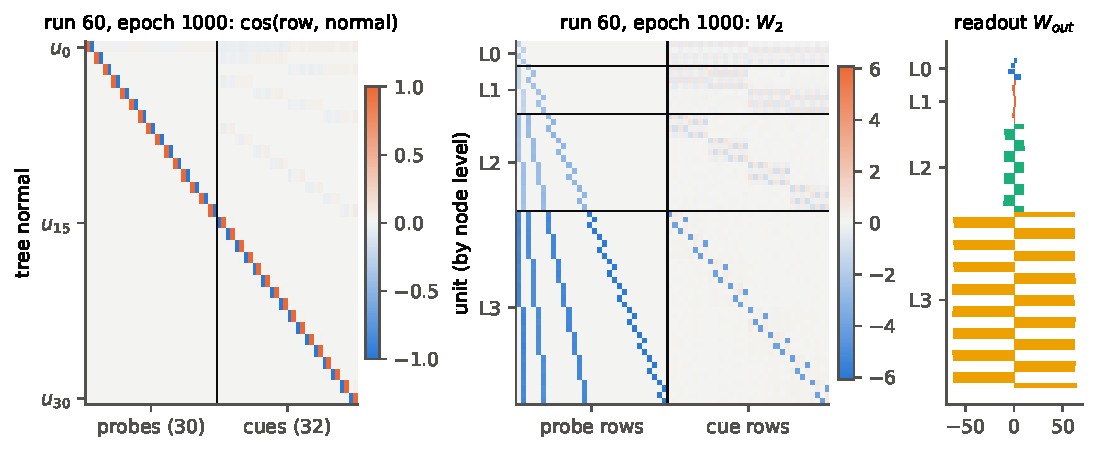
\includegraphics[width=\textwidth]{figs/learned_run60.pdf}
\caption{Run 60 at epoch 1000. Left: every probe is $\pm u_j$ and every cue $\pm u_m$. Middle: $W_2$; the level-3 units veto their own probe and the probes of their ancestors (the diagonal bands), and the cue block has become a one-cue-per-unit pattern. Right: readouts by level; the level-3 units dominate.}
\label{fig:learned}
\end{figure}

\begin{figure}[!htbp]\centering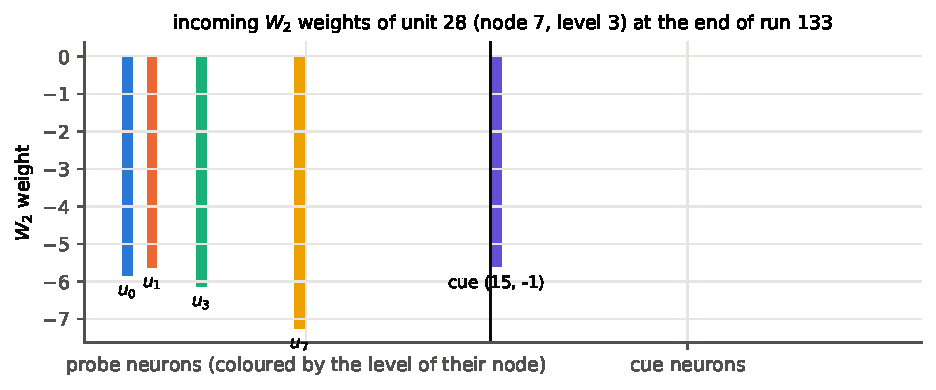
\includegraphics[width=\textwidth]{figs/unit_example.pdf}
\caption{Incoming weights of one level-3 unit (unit 28, node 7) at the end of run 60: vetoes of $-5$ to $-6$ on its own probe and on one probe of each ancestor ($u_3$, $u_1$, $u_0$), a veto of $-4$ on the opposite-pole cue of leaf 15, and small positive weights on the other cues (the background).}
\label{fig:unit}
\end{figure}

\section{Symmetrised gradients: simulating population gradient flow}
\label{sec:sym}
\paragraph{The group.} Let $G$ be generated by the 15 flips $F_j$ (negate $u_j$, exchange the two subtrees below $j$) and the label negation $N$ (negate the 16 leaf normals, which negates $y$); $|G|=2^{16}=65\,536$. Each $g\in G$ acts on the parameters by permuting the rows according to their identities (probe $(j,\pm)$, cue $(m,\pm)$), permuting the units according to theirs (node, block sign, path sign), and flipping the signs of the affected coordinates of $W_1$ and of $W_{\mathrm{out}}$. The loss is invariant, $L(g\cdot\theta)=L(\theta)$, and the designed initialisations are fixed points, $g\cdot\theta_0=\theta_0$. Gradient flow on the population loss therefore stays on the fixed-point set forever; finite-sample SGD leaves it at the first step.

\paragraph{The symmetrised flow.} We run the same SGD but project every minibatch gradient onto the symmetric subspace: coordinates of $(W_1,W_2,W_{\mathrm{out}})$ are grouped into orbits of $G$ (with signs), each gradient entry is replaced by the signed mean over its orbit, and orbits that contain a coordinate and its own negative are set to zero. This equals the gradient on the minibatch augmented by all $65\,536$ images of its points, at the cost of one backward pass and a bincount. Of the $7\,562$ coordinates, 203 orbits remain, 157 of them free (Figure~\ref{fig:orbits}); a probe's in-span part, for instance, can only move along its own normal and the normals of its ancestors. Sampling noise survives only inside this subspace, so the trajectory is an estimate of the population flow from the symmetric init, with the usual step-size discretisation.

\begin{figure}[!htbp]\centering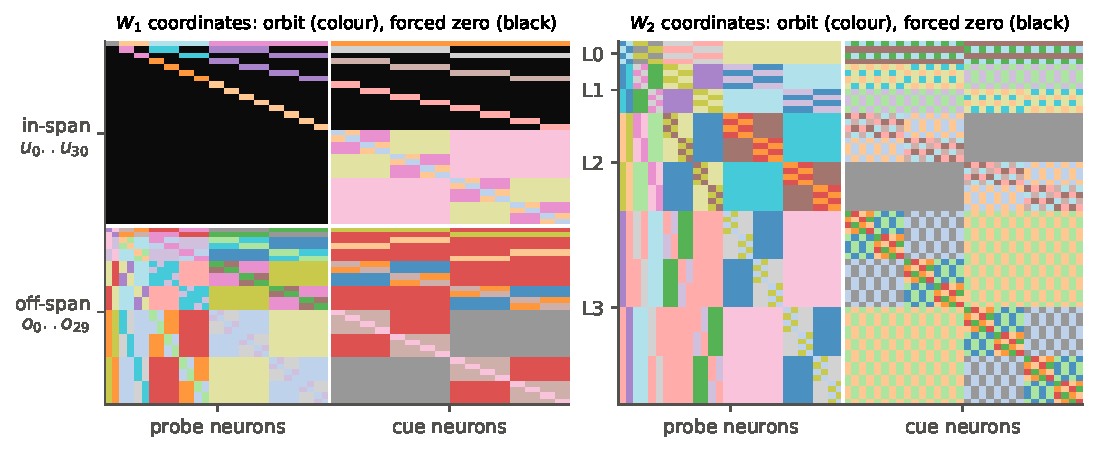
\includegraphics[width=\textwidth]{figs/orbits.pdf}
\caption{Orbit structure of the parameter coordinates (colour = orbit; colours repeat, black = forced to zero). In $W_1$, the in-span coordinates of a probe are free only on its own normal and its ancestors' (the staircase in the top-left block), the cues' in-span coordinates on the leaf normals, and all off-span coordinates are free. In $W_2$ every block is free, tied across the units of a level.}
\label{fig:orbits}
\end{figure}

\paragraph{Run 74: the flow from run 60's init.} The symmetrised run from run 60's initialisation captures the levels at epochs 9, 15, 21, 30 (SGD: 10, 40, 22, 31), rotates the cues by epoch 801 (SGD: 653) and ends at $0.029$ loss and $0.45\,\%$ error (Figure~\ref{fig:traj74}, left panel of Figure~\ref{fig:overlay}). On this init, SGD and the population flow agree: the design's pushes are 30--40 times the sampling noise, so the noise is irrelevant. Run 114 repeats run 74 with the cosine schedule restarted at the unfreeze epoch and reaches $0.006$ loss and $0.05\,\%$ error; the cold second half of a single cosine was the only thing holding run 74 back.

\paragraph{Runs 73 and 97: the flow from run 70's init.} Here the two differ. SGD (run 70) captured only the root; the symmetrised flow (run 73, with the frozen phase doubled to 1000 epochs) captures all four levels, at epochs 98, 408, 313, 396, every probe on its own node (Figure~\ref{fig:traj7397}, right panel of Figure~\ref{fig:overlay}). The small side contrast of run 70's weights gives pushes only a few times the sampling noise, and under SGD the probes of levels 1--3 are decided by the sample: they climb to the root or to an ancestor. Under the population flow the same wiring is enough. Run 73's cues did not rotate within its cold free phase; run 97 continues it for 2000 epochs with a fresh cosine and the cues rotate within 23 epochs, ending at $0.010$ loss and $0.11\,\%$ error with all 31 normals covered. The lesson is that the design's mechanism is deterministic and complete, and that the failures of SGD on the weaker init are symmetry breaking by sampling, not a missing ingredient.

\begin{figure}[!htbp]\centering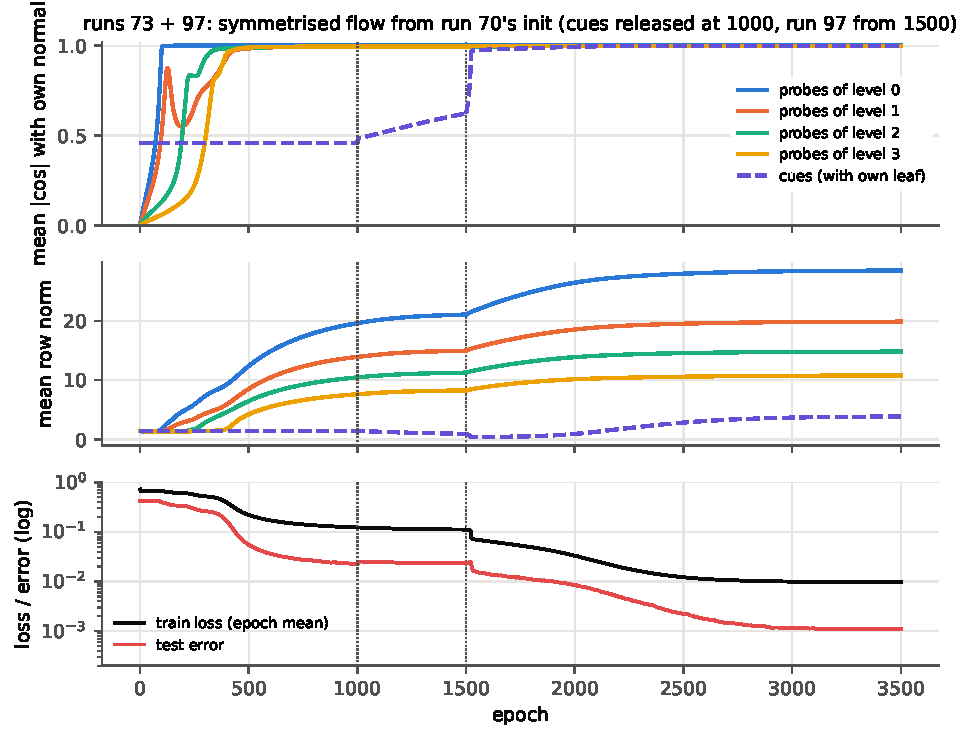
\includegraphics[width=0.9\textwidth]{figs/traj_run73_97.pdf}
\caption{Runs 73 and 97 (symmetrised flow from run 70's init). Every level is captured during the frozen phase (root at 98, levels 1--3 by 408), with the transient dips of levels 1--2 showing the competition between a node and its ancestors that the symmetric flow resolves in favour of the node. The cues rotate only once run 97 restarts the learning rate (epoch 1500); loss and error then fall by an order of magnitude.}
\label{fig:traj7397}
\end{figure}

\begin{figure}[!htbp]\centering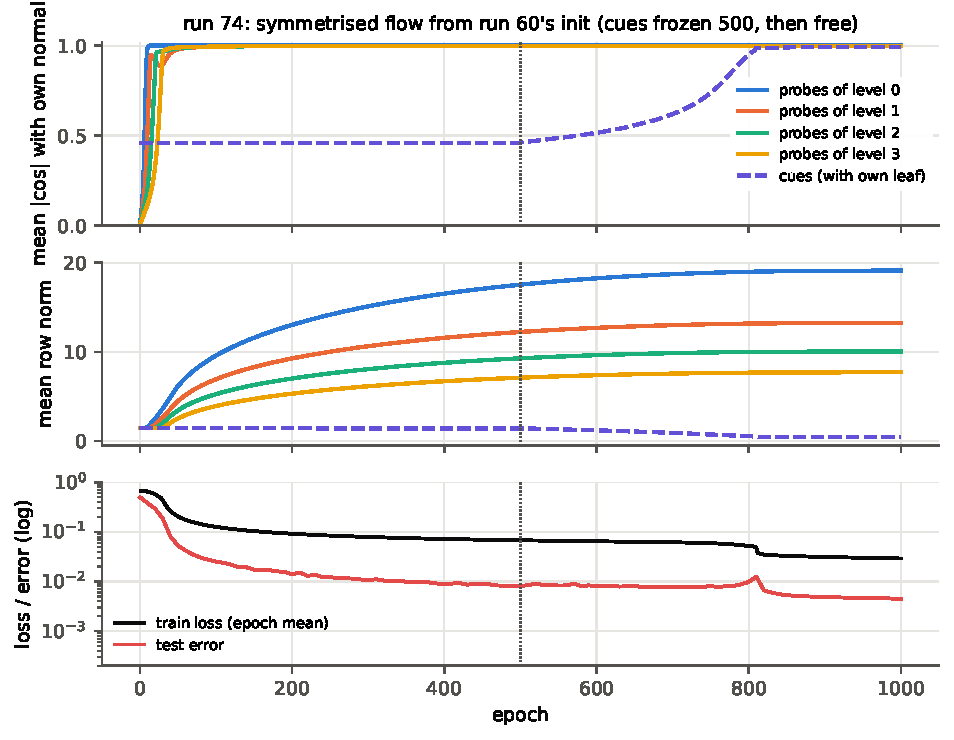
\includegraphics[width=0.9\textwidth]{figs/traj_run74.pdf}
\caption{Run 74 (symmetrised flow from run 60's init). Indistinguishable from run 60 at the level of these curves.}
\label{fig:traj74}
\end{figure}

\begin{figure}[!htbp]\centering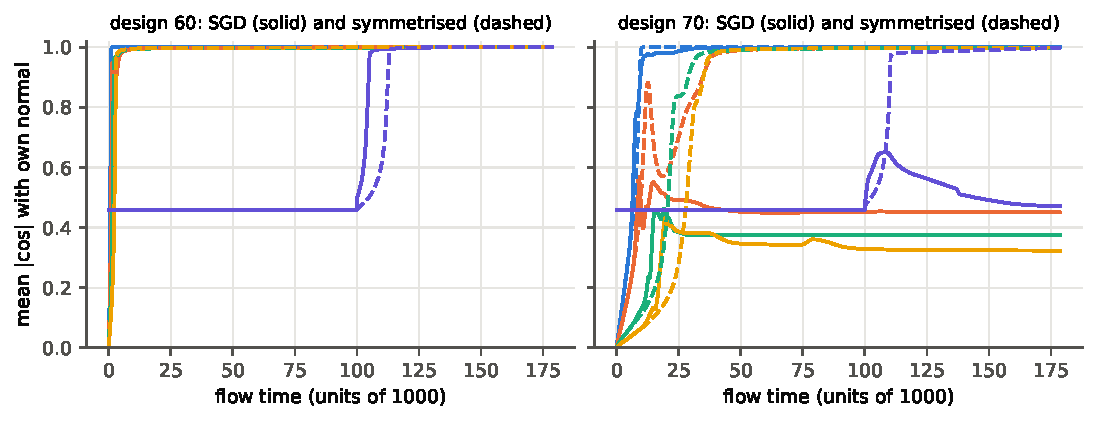
\includegraphics[width=\textwidth]{figs/overlay_sgd_vs_sym.pdf}
\caption{SGD against the symmetrised flow. Left: run 60 and run 74 coincide. Right: run 70 loses levels 1--3 to noise-driven competition, run 73 captures them all.}
\label{fig:overlay}
\end{figure}

\section{What this buys, and where it is going}
\begin{itemize}[leftmargin=1.4em,itemsep=2pt]
\item \textbf{A mechanism, not a correlation.} The lens formula \eqref{eq:lens} predicts which row moves along which normal from the wiring alone, including the order (root first, because the side contrast of a level-$l$ block sums over $2^{4-l}$ leaves) and the transient ancestor components. The symmetrised runs show the mechanism works without any help from noise.
\item \textbf{The ``cheating'' budget is explicit.} The init uses the tree in three places: the cue bias $\beta$, the side contrast, and the absence of off-span components in the cues. Each is now one scalar of the $\alpha$ parametrisation and has been swept (notebook 2, sections 34--38). The flow restores the third by itself within tens of epochs, the first costs time like $1/\beta$ with no threshold in the population flow, and the second is the one quantity gradient descent does not create from a side-symmetric start.
\item \textbf{The open theoretical question} is the random-init version of this story: a random first layer has a small component of order $0.1$ on every routing normal, a random $W_2$ reads the two sides of a node unequally by chance, and the loop ``probe component on $u_j$ $\to$ cue side contrast on $j$ $\to$ probe push on $j$'' is a per-node instability of the symmetric state whose growth rates should be ordered by level. Making that precise, and testing it with large-batch GD from random inits, is the next line of work.
\end{itemize}

\paragraph{Where things are in the repository.}
Code: \path{src/layer_lenses/alpha_init.py} (the $\alpha$ parametrisation of the inits), \path{symmetric_flow.py} (orbits and projection), \path{run_analysis.py} and \path{path_analysis.py} (trajectory and path tools). Runners: \path{results/designed_init/run_hd2_phased.py} (SGD runs such as 60 and 70) and \path{run_symmetric_gd.py} (symmetrised runs such as 73, 74, 97, 114). Notebooks: \path{notebooks/hierarchy_design_runs_2.ipynb} (one section per run, with findings) and \path{notebooks/two_layer_network_anatomy.ipynb} (choose a run and an epoch; the replay trajectories of runs 60, 70, 73 and 74 are in the repository). Notes: \path{notes/session_log.md} is the chronological record; this handout and the script that made its figures are in \path{notes/handout/}.
\end{document}
